\documentclass[dcc]{fcfmcourse}
\usepackage{teoria}
\usepackage[utf8x]{inputenc}
\usepackage{amsmath}
\usepackage{amsfonts,setspace}
\usepackage{listings}
\usepackage{color}
\usepackage{cancel}
\usepackage{epstopdf}
\usepackage{qtree}
\usepackage{fancyhdr}
\usepackage{tikz}
\usetikzlibrary{automata,positioning}
\pagestyle{fancy}
\cfoot{``You need the willingness to fail all the time" \\John Backus}
\definecolor{pblue}{rgb}{0.13,0.13,1}
\definecolor{pgreen}{rgb}{0,0.5,0}
\definecolor{porange}{rgb}{0.9,0.5,0}
\definecolor{pgrey}{rgb}{0.46,0.45,0.48}

\lstset{language=Java,
  showspaces=false,
  showtabs=false,
  breaklines=true,
  showstringspaces=false,
  breakatwhitespace=true,
  commentstyle=\color{porange},
  keywordstyle=\color{pblue},
  stringstyle=\color{pgreen},
  basicstyle=\ttfamily,
  moredelim=[il][\textcolor{pgrey}]{$ $},
  moredelim=[is][\textcolor{pgrey}]{\%\%}{\%\%}
}

\newenvironment{codebox} {\small \ttfamily \obeylines \begingroup \setstretch{-2.4}} {\endgroup}

\title{Auxiliar 5}
\course[CC3102]{Teoría de la Computación}
\professor{Gonzalo Navarro}
\assistant{Manuel Cáceres}
\assistant{Ian Letter}

% Si pasas el comando usedate a la clase, la fecha aparecerá bajo la lista de auxiliares.
% Puedes usar el formato de fecha por defecto de latex (y traducirla usando babel)
% o puedes escribir lo que quieras con el comando \date.
% \date{1 de Septiembre, 2015}

\begin{document}
\maketitle
\begin{center}
5 de Octubre del 2016
\end{center}
\vspace{-1ex}

\section*{Gramáticas Libres del Contexto}
\begin{problems}
\problem Demuestre que el lenguaje de la gramática 
\begin{center}
$S \rightarrow \epsilon\, | aSbS\,| bSaS$
\end{center}
Es $\{w \in \{a,b\}^*\,\colon \#_{a}(w)=\#_{b}(w)\}$
\problem Encuentre una GLC para los siguientes lenguajes:
\begin{enumerate}[a)]
    \item $\{ww^R\colon w \in\{a,b\}^*\}$
    \item $\{w \in \{a,b\}^*\,\colon w=w^R\}$
    \item $\{a,b\}^* \setminus \{ww\colon w \in\{a,b\}^*\}$
\end{enumerate}
\end{problems}

\section*{Ambigüedad}
\begin{problems}
\problem Para las siguientes gramáticas describa el lenguaje que genera, muestre que es ambigua y de una gramática alternativa no ambigua:

\begin{enumerate}[a)]
    \item $S \rightarrow \epsilon\, | SS\,| (S)$
    \item $S \rightarrow \epsilon\, | if\, S\,| if\, S\, else\, S$
\end{enumerate}
\end{problems}

\section*{Autómatas de Pila}
\begin{problems}
\problem Construya autómatas de pila para los siguientes lenguajes:
\begin{enumerate}[a)]
    \item $\{w \in \{a,b\}^*\,\colon \#_{a}(w)=\#_{b}(w)\}$
    \item $\{ww^R\colon w \in\{a,b\}^*\}$
    \item $\{w \in \{a,b,c\}^*\,\colon w=w^R\}$. ¿Puede hacerlo con solo dos caracteres en la pila?
    \item $\{w\$v\colon w\not = v\, y \, w,v \in\{a,b\}^*\}$
\end{enumerate}
\end{problems}
\newpage
\begin{center}
{\huge \underline{Soluciones}}
\end{center}
\section*{Gramáticas Libres del Contexto}
\begin{problems}
\problem
Para mostrar que el lenguaje generado por la gramática es exactamente  el lenguaje descrito debemos mostrar dos cosas :
\begin{enumerate}[1.]
\item \textbf{Todo string derivado de la gramática está en el lenguaje.}\\
En este caso es simple ver que un $w$ derivado de la gramática cumple que $\#_{a}(w)=\#_{b}(w)$, pues las reglas de derivación generan $a$'s y $b$'s de a pares\footnote{Una demostración formal haría inducción usando las reglas de la gramática y mostrando que $\#_{a}(w)=\#_{b}(w)$ se mantiene para cada una de ellas.}.
\item \textbf{Todo string en el lenguaje se puede derivar de la gramática.}\\
Para esto consideremos un $w$ tal que $\#_{a}(w)=\#_{b}(w)$, debemos mostrar que existe una derivación de $w$ en la gramática.\\

Sin mucha pérdida de generalidad suponemos que $w$ comienza con una $a$ (si es la cadena vacía, tenemos la derivación correspondiente y si empieza con $b$ el razonamiento que daremos a continuación es análogo).\\

Como $w$ comienza con una $a$ la única regla que podemos usar para derivar $w$ es $S \rightarrow  aSbS$, lo que nos queda mostrar es que podemos escribir \underline{$w = axby$, con $x, y \in \mathcal{L}$}, pues si lo logramos, podemos utilizar la regla de derivación $aSbS$ y aplicar inductivamente este argumento sobre $x$ e $y$.\\

Para demostrar lo anterior definimos $w_{i}$ como el prefijo de largo $i$ de $w$, en particular tenemos que $w_{1}=a$ y $w_{|w|}=w$.\\
Sea $k$ el mínimo valor tal que $\#_{a}(w_{k})=\#_{b}(w_{k})$ (existe pues $k=|w|$ lo cumple).\\
Estudiemos la sucesión $(\#_{a}(w_{i})-\#_{b}(w_{i}))_{i\in \{1,\ldots, |w|\}}$, de ella sabemos que :
\begin{itemize}
\item Su primer valor es 1, pues $\#_{a}(a)-\#_{b}(a) = 1-0 = 1$
\item El primer índice en el que vale 0 es $k$, pues $k$ es el el mínimo valor tal que $\#_{a}(w_{k})=\#_{b}(w_{k})$
\item Su último valor es 0, pues $\#_{a}(w)=\#_{b}(w)$
\end{itemize}
De este modo la sucesión se ve como $(1_{1},\ldots,0_{k},\ldots,0_{|w|})$. De ella podemos deducir que la última letra de $w_{k}$ es una $b$, puesto que si fuese una $a$ el $(k-1)$-ésimo término de la sucesión sería $-1$ (que no es posible pues la primera aparición de $0$ es en $k$).\\
Entonces $w = w_{k}y = axby$, y como $\#_{a}(w_{k})=\#_{b}(w_{k})$ entonces $\#_{a}(x)=\#_{b}(x)$ y además $\#_{a}(y)=\#_{b}(y)$, con lo que $x,y \in \mathcal{L}$.
\end{enumerate}
\newpage
\problem
\begin{enumerate}[a)]
\item $S \rightarrow \epsilon\, | aSa\,| bSb$
\item $S \rightarrow \epsilon\, | a\, | b\, | aSa\,| bSb$
\item Gramática con las siguientes reglas :
\begin{center}
$S \rightarrow A\, | B\, | AB\, | BA$\\
$A \rightarrow a\, | aAa\, | aAb\, | bAb\,| bAa$\\
$B \rightarrow b\, | aBa\, | aBb\, | bBb\,| bBa$
\end{center}
Veamos ahora que el lenguaje generado por esta gramática es exactamente $\mathcal{L}$.\\

Antes de hacer la demostración, observemos que las palabras derivadas por $A$ son las palabras de largo impar que tienen una $a$ en el centro y las derivadas por $B$ son las de largo impar que tienen una $b$ en el centro, luego las por derivadas por $A|B$ son todas las palabras de largo impar, las cuales están en el lenguaje. Y por otro lado, si está en el lenguaje y es de largo impar, es esta regla la que deriva la cadena.\\
De esta manera, la demostración siguiente será realizada asumiendo que el largo de $w$ es par.\\
\begin{enumerate}[1.]
\item \textbf{Todo string en el lenguaje se puede derivar de la gramática.}\\
Sea $w = w_{1}w_{2}\ldots w_{n}$ en el lenguaje, por lo tanto $\exists i, w_{i} \not = w_{i+n/2}$ (si no $w$ sería de la forma $xx$).\\
Consideremos $w_{1}\ldots w_{2i-1}$ y $w_{2i}\ldots w_{n}$, las cuales son dos secuencias de largo impar tales que sus letras centrales ($w_{i}$ y $w_{i+n/2}$) son diferentes, por lo que puede ser derivada según la regla $AB|BA$.
\item \textbf{Todo string derivado de la gramática está en el lenguaje.}\\
Supongamos ahora que $w$ es un string derivado de la gramática. Como $w$ es de largo par, debe haber sido derivado de $AB|BA$. Sin mucha pérdida de generalidad supongamos que fue derivado de la regla $AB$ (el razonamiento es el mismo en el otro caso), es decir $w=uv$ con $u$ derivable de $A$ y $v$ derivable de $B$.\\

Si $|u|=|v|$, entonces $u \not = v$, pues tienen diferente letra central ($u$ una $a$ y $v$ una $b$).\\
En el caso en que los largos no son iguales definimos $l=|u|$ y por lo tanto $|v| = n-l$.\\
En este caso sus letras centrales son $u_{(l+1)/2}$ y $v_{(n-l+1)/2}$ respectivamente, que sabemos que son diferentes (una es una $a$ y la otra una $b$). Pero esto significa que $w_{(l+1)/2} \not = w_{(n+l+1)/2}$.\\
Finalmente si separo $w = xx'$ en cadenas $|x|=|x'|$ tengo que $x_{(l+1)/2} = w_{(l+1)/2} \not = w_{(n+l+1)/2} = x_{(l+1)/2}'$ por lo que $x \not = x'$.\footnote{Notemos que este caso es independiente de $u \not = v$.}
\end{enumerate}
\end{enumerate}
\end{problems}
\newpage
\section*{Ambigüedad}
\begin{problems}
\problem 
\begin{enumerate}[a)]
\item El lenguaje derivado es el de los paréntesis balanceados. La cadena $()()()$ tiene dos árboles de derivación diferentes :
\begin{center}
\begin{tabular}{c c}
\Tree [.S [.S [.S () ] [.S () ] ] [.S () ]  ]  & \Tree [.S [.S [.S () ] [.S () ] ] [.S () ]  ]
\end{tabular}
\end{center}
Por lo que es ambigua.\\
Una gramática no ambigua es : 
\begin{center}
$S \rightarrow (RS\, | \epsilon$\\
$R \rightarrow )\, | (RR$\\
\end{center}
La $R$ deriva los strings que tienen un paréntesis derecho más que un izquierdo. Como intuición la gramática no es ambigua pues si recorro unos paréntesis balanceados de izquierda a derecha, siempre voy a poder ocupar una única regla.

\item El lenguaje derivado es el de los programas sintácticamente bien escritos a los cuales se les borraron todas las sentencias excepto los \textit{keywords} $if$ y $else$. La cadena $if\ if\ else$ tiene dos árboles de derivación distintos :
\begin{center}
\begin{tabular}{c c}
\Tree [.S $if$ [.S $if$ [.S $\epsilon$ ] $else$ [.S $\epsilon$ ] ] ]  & \Tree [.S $if$ [.S $if$ [.S $\epsilon$ ] ] $else$ [.S $\epsilon$ ] ]
\end{tabular}
\end{center}
Por lo que es ambigua.\\
Una gramática no ambigua es : 
\begin{center}
$S \rightarrow \epsilon\, | if\ B\ else\ S\, | if\ S$\\
$B \rightarrow if\ B\ else\ B\, | \epsilon$\\
\end{center}
La intuición aquí es que el conjunto podemos \textbf{particionarlo} en tres; la cadena vacía, aquellas cadenas que cierran su primer $if$ con un $else$ y aquellas cadenas que no cierran su primer $if$. Como lo anterior construye derivaciones no ambiguas para cada uno de estos tipos de cadenas, entonces la gramática no es ambigua.
\end{enumerate}
\end{problems}
\newpage
\section*{Autómatas de Pila}
\begin{problems}
\problem 
\begin{enumerate}[a)]
\item 
Este autómata :\\

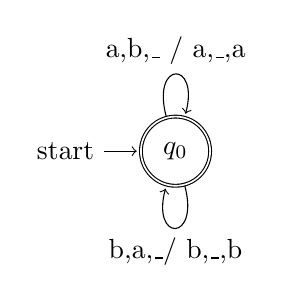
\begin{tikzpicture}[shorten >=1pt,node distance=2cm,on grid,auto] 
   \node[state,initial,accepting] (q_0)   {$q_0$}; 
    \path[->] 
    (q_0) edge [loop above] node  {a,b,\_\ /\ a,\_,a} (q_0)
    (q_0) edge [loop below] node  {b,a,\_\\ /\ b,\_,b} (q_0);
\end{tikzpicture}
\item 
Este autómata :\\

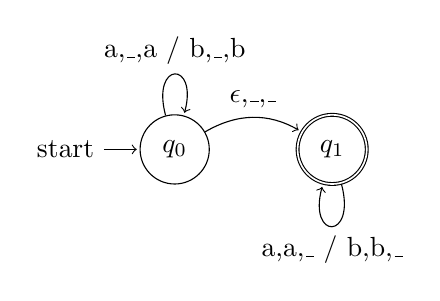
\begin{tikzpicture}[shorten >=1pt,node distance=2cm,on grid,auto] 
   \node[state,initial] (q_0)	{$q_0$}; 
   \node[state,accepting] (q_1) [right of=q_0]  {$q_1$}; 
    \path[->] 
    (q_0) edge [loop above] node  {a,\_,a\ /\ b,\_,b} (q_0)
    (q_0) edge [bend left] node  {$\epsilon$,\_,\_} (q_1)
    (q_1) edge [loop below] node  {a,a,\_\ /\ b,b,\_} (q_1);
\end{tikzpicture}
\item 
Este autómata :\\

    \begin{tikzpicture}[shorten >=1pt,node distance=10cm,on grid,auto] 
       \node[state,initial] (q_0)	{$q_0$}; 
       \node[state,accepting] (q_1) [right of=q_0]  {$q_1$}; 
        \path[->] 
        (q_0) edge [loop above] node  {a,\_,a\ /\ b,\_,b\ /\ c,\_,c} (q_0)
        (q_0) edge [bend left] node  {$\epsilon$,\_,\_\ /\ a,\_,\_\ /\ b,\_,\_\ /\ c,\_,\_} (q_1)
        (q_1) edge [loop below] node  {a,a,\_\ /\ b,b,\_\ /\ c,\_,c} (q_1);
    \end{tikzpicture}
\newpage
\item 
Este autómata :\\

\begin{center}
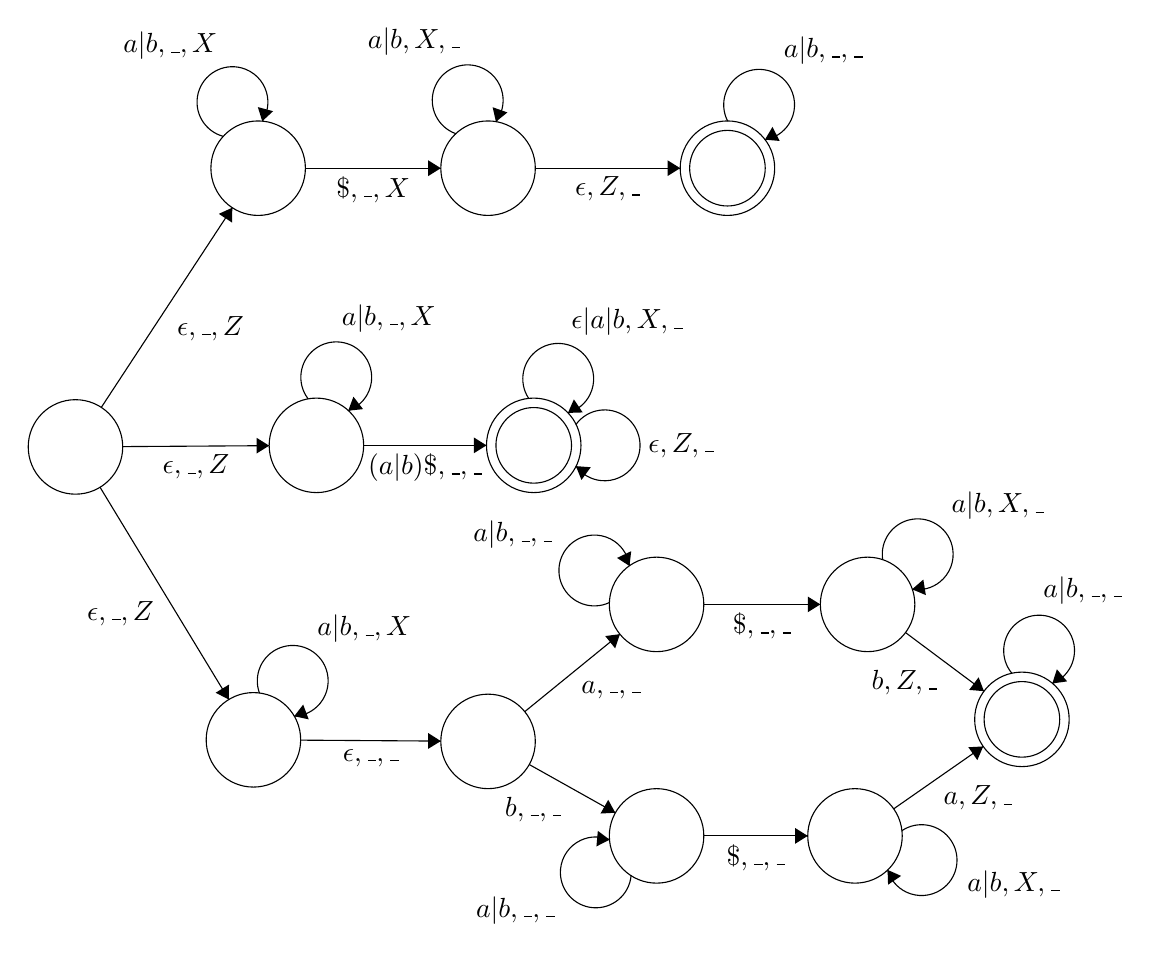
\begin{tikzpicture}[scale=0.2]
\tikzstyle{every node}+=[inner sep=0pt]
\draw [black] (9.8,-28.4) circle (3);
\draw [black] (21.4,-10.7) circle (3);
\draw [black] (25.1,-28.3) circle (3);
\draw [black] (21.1,-47) circle (3);
\draw [black] (36,-47.1) circle (3);
\draw [black] (46.7,-38.4) circle (3);
\draw [black] (46.7,-53.1) circle (3);
\draw [black] (60.1,-38.4) circle (3);
\draw [black] (59.3,-53.1) circle (3);
\draw [black] (69.9,-45.7) circle (3);
\draw [black] (69.9,-45.7) circle (2.4);
\draw [black] (36,-10.7) circle (3);
\draw [black] (51.2,-10.7) circle (3);
\draw [black] (51.2,-10.7) circle (2.4);
\draw [black] (38.9,-28.3) circle (3);
\draw [black] (38.9,-28.3) circle (2.4);
\draw [black] (11.36,-30.96) -- (19.54,-44.44);
\fill [black] (19.54,-44.44) -- (19.55,-43.49) -- (18.7,-44.01);
\draw (14.81,-38.97) node [left] {$\epsilon,\_,Z$};
\draw [black] (12.8,-28.38) -- (22.1,-28.32);
\fill [black] (22.1,-28.32) -- (21.3,-27.82) -- (21.3,-28.82);
\draw (17.45,-28.87) node [below] {$\epsilon,\_,Z$};
\draw [black] (11.44,-25.89) -- (19.76,-13.21);
\fill [black] (19.76,-13.21) -- (18.9,-13.6) -- (19.74,-14.15);
\draw (16.22,-20.87) node [right] {$\epsilon,\_,Z$};
\draw [black] (21.486,-44.037) arc (200.30993:-87.69007:2.25);
\draw (28.14,-40.88) node [above] {$a|b,\_,X$};
\fill [black] (23.69,-45.5) -- (24.61,-45.7) -- (24.26,-44.76);
\draw [black] (24.1,-47.02) -- (33,-47.08);
\fill [black] (33,-47.08) -- (32.2,-46.57) -- (32.2,-47.57);
\draw (28.55,-47.57) node [below] {$\epsilon,\_,\_$};
\draw [black] (38.33,-45.21) -- (44.37,-40.29);
\fill [black] (44.37,-40.29) -- (43.44,-40.41) -- (44.07,-41.19);
\draw (43.81,-43.24) node [below] {$a,\_,\_$};
\draw [black] (38.62,-48.57) -- (44.08,-51.63);
\fill [black] (44.08,-51.63) -- (43.63,-50.81) -- (43.14,-51.68);
\draw (38.86,-50.6) node [below] {$b,\_,\_$};
\draw [black] (49.7,-38.4) -- (57.1,-38.4);
\fill [black] (57.1,-38.4) -- (56.3,-37.9) -- (56.3,-38.9);
\draw (53.4,-38.9) node [below] {$\$,\_,\_$};
\draw [black] (49.7,-53.1) -- (56.3,-53.1);
\fill [black] (56.3,-53.1) -- (55.5,-52.6) -- (55.5,-53.6);
\draw (53,-53.6) node [below] {$\$,\_,\_$};
\draw [black] (61.76,-51.38) -- (67.44,-47.42);
\fill [black] (67.44,-47.42) -- (66.5,-47.47) -- (67.07,-48.29);
\draw (67.1,-49.9) node [below] {$a,Z,\_$};
\draw [black] (62.51,-40.19) -- (67.49,-43.91);
\fill [black] (67.49,-43.91) -- (67.15,-43.03) -- (66.55,-43.83);
\draw (62.45,-42.55) node [below] {$b,Z,\_$};
\draw [black] (24.4,-10.7) -- (33,-10.7);
\fill [black] (33,-10.7) -- (32.2,-10.2) -- (32.2,-11.2);
\draw (28.7,-11.2) node [below] {$\$,\_,X$};
\draw [black] (33.963,-8.513) arc (250.69924:-37.30076:2.25);
\draw (31.3,-3.57) node [above] {$a|b,X,\_$};
\fill [black] (36.5,-7.75) -- (37.23,-7.16) -- (36.29,-6.83);
\draw [black] (39,-10.7) -- (48.2,-10.7);
\fill [black] (48.2,-10.7) -- (47.4,-10.2) -- (47.4,-11.2);
\draw (43.6,-11.2) node [below] {$\epsilon,Z,\_$};
\draw [black] (28.1,-28.3) -- (35.9,-28.3);
\fill [black] (35.9,-28.3) -- (35.1,-27.8) -- (35.1,-28.8);
\draw (32,-28.8) node [below] {$(a|b)\$,\_,\_$};
\draw [black] (19.196,-8.682) arc (255.25051:-32.74949:2.25);
\draw (15.82,-3.84) node [above] {$a|b,\_,X$};
\fill [black] (21.66,-7.72) -- (22.35,-7.08) -- (21.38,-6.82);
\draw [black] (43.714,-38.278) arc (295.38954:7.38954:2.25);
\draw (40.1,-33.98) node [left] {$a|b,\_,\_$};
\fill [black] (44.98,-35.96) -- (45.09,-35.02) -- (44.19,-35.45);
\draw [black] (45.083,-55.613) arc (-5.03624:-293.03624:2.25);
\draw (40.27,-57.84) node [left] {$a|b,\_,\_$};
\fill [black] (43.72,-53.34) -- (42.97,-52.78) -- (42.88,-53.77);
\draw [black] (61.06,-35.57) arc (189:-99:2.25);
\draw (65.4,-32.15) node [right] {$a|b,X,\_$};
\fill [black] (62.93,-37.44) -- (63.8,-37.81) -- (63.64,-36.82);
\draw [black] (62.27,-52.773) arc (124.01689:-163.98311:2.25);
\draw (66.4,-56.19) node [right] {$a|b,X,\_$};
\fill [black] (61.37,-55.26) -- (61.4,-56.2) -- (62.23,-55.64);
\draw [black] (24.581,-25.357) arc (217.7398:-70.2602:2.25);
\draw (29.7,-21.15) node [above] {$a|b,\_,X$};
\fill [black] (27.12,-26.1) -- (28.06,-26) -- (27.45,-25.21);
\draw [black] (38.585,-25.328) arc (213.77514:-74.22486:2.25);
\draw (44.82,-21.37) node [above] {$\epsilon|a|b,X,\_$};
\fill [black] (41.07,-26.24) -- (42.01,-26.21) -- (41.45,-25.38);
\draw [black] (69.267,-42.78) arc (219.96376:-68.03624:2.25);
\draw (73.77,-38.43) node [above] {$a|b,\_,\_$};
\fill [black] (71.83,-43.42) -- (72.77,-43.29) -- (72.12,-42.52);
\draw [black] (51.216,-7.712) arc (207.43495:-80.56505:2.25);
\draw (57.29,-4.15) node [above] {$a|b,\_,\_$};
\fill [black] (53.58,-8.89) -- (54.52,-8.97) -- (54.06,-8.08);
\draw [black] (41.58,-26.977) arc (144:-144:2.25);
\draw (46.15,-28.3) node [right] {$\epsilon,Z,\_$};
\fill [black] (41.58,-29.62) -- (41.93,-30.5) -- (42.52,-29.69);
\end{tikzpicture}
\end{center}

\end{enumerate}
\end{problems}
\end{document}
